% \subsection{Detailed Introduction}
% Describe in more details the work done: The physics, the models. The specific
% litterature search goes here.

The previous section described the general goals of this thesis and was used to
give the reader an overview picture of the field. The following will go
into more details.

\subsection{Goals}
In view of the previous section, the goal of the current thesis is to increase
to global knowledge of laser-matter interaction. More specifically, the
question of \textit{how} the energy is deposited in a nanoscale object by an
ultra-short and ultra-intense laser pulse is important.

\cite{Young2010,Chapman2011}

\subsection{Laser-Cluster interaction}


\subsubsection{Clusters}
\label{section:intro:clusters:clusters}

Clusters of atoms are an extremely useful tool to study laser-matter
interaction. They are experimentally easy to produce since many
years\cite{Haberland1994}. Their size and constitution can be varied almost at
will \cite{Martin1996}.

\cite{Fennel2010}

\subsubsection{Heating mechanisms}
\label{section:intro:clusters:heating}

\subsubsection{Studied parameters}


\subsection{Methodology and Tools}
A large selection of tools exist to study laser-cluster interaction,
differentiating themselves through the amount of approximation taken.

Exact solution of the quantum mechanical system is, most of the time,
intractable. Theoretical investigations thus require some degree of
approximation, a compromise between feasibility and exactitude. On one end of
the spectrum, the most general methods is solving the
Time-Dependent \schrodinger Equation (TDSE) directly or the Quantum Monte-Carlo
(QMC) method. Unfortunately, these methods can only be applied to the simplest
systems of small numbers of electrons; clusters cannot be studied using these
methods.

Larger systems can be studied using \textit{ab initio} methods (``from
first principles'') which covers a wide range of techniques. In this class of
methods one can find \textit{Hartree-Fock} (HF) methods which consist on
approximating the ground state wavefunction by a single Slater determinant.
In HF methods, instantaneous electron-electron Coulomb repulsion is not
included directly in the system's Hamiltonian. Instead, only the average field
resulting from other electrons is used, giving the often used name of
\textit{self-consistent field} methods. Other \textit{ab
initio} methods are the \textit{Post Hartree-Fock} methods where electron
correlation is added. An example is the \textit{Configuration Interaction} (CI)
method. Because of their great accuracy, these methods are restricted to
relatively small systems, generally less then 10 atoms. Full \textit{ab initio}
treatment of clusters is not possible.

Larger systems requires more approximations. \textit{Density Functional Theory}
is an often used method for cluster studies requiring quantum aspects, with
either quantum or semiclassical propagation. It starts by formulating an
expression for the total energy of electrons and ions and derives static and
dynamic equations from it. All approximations are done in the selection of this
(energy) functional. The upper limit on these methods is of practical reasons,
mainly computational power available. On the other side, because the chosen
functional approximate the underlying quantum system, specific quantum effects
might not be included, for example shell effects or tunnelling are neglected.

Because DFT methods are mean field in nature, they cannot account for the large
field fluctuations seen in strong field cluster dynamics.

On the end of the methods spectrum lies the rate equations.






For a detailed review of the different methods, see Ref. \cite{Fennel2010}.



\subsubsection{Molecular Dynamics (MD)}
Due to the high charge states seen in experiment with clusters the only
practical method to microscopically study the ionization dynamics is
\textit{Molecular Dynamics} (MD) methods where ions and electrons are treated
classically.

In MD, particles interact directly through classical instantaneous forces. The
total force acting on particle $i$ of mass $m_i$ from all other $N$ particles in
the system is:
\begin{align}
m_i \va_i & = \vF_i = \sum_{j \ne i} \vF_{j \rightarrow i}
\label{eqn:md:newton}
\end{align}
In the present work, the force between charged particles is the instantaneous
electrostatic Coulomb force:
\begin{align}
\vF_{C,j \rightarrow i}\pa{\vr} & =\frac{k q_i q_j}{r_{ji}^2} \hvr_{ji}.
\label{eqn:md:coulomb:F}
\end{align}
which only depends on the distance between particles. Figure
\ref{fig:md:vectors} shows the vectors definition used throughout this work. We
define particle $i$ the particle we are interested in (for example, the
particle we are calculating the force on), and particle $j$ the particle that
is generating the field or potential that is measured at location $i$. We thus
have:
\begin{align}
\vr_{j} + \vr_{j,i} & = \vr_{i} \\
\vr_{j,i} & = \vr_{i} - \vr_{j}
\end{align}
%       _j
%       /|\
%  r_j /   \ r_ji
%     /    _\/
%    /------>i
%       r_i

\emptyfig{Vectors definition}{fig:md:vectors}


Equation \eqref{eqn:md:newton} can be time integrated using the
Velocity-Verlet (VV) scheme:
\begin{subequations}
\begin{align}
\vx_{i}^{\pa{n+1}} & = \vx_{i}^{\pa{n}} + \vv_{i}^{\pa{n}} \Delta t +
\frac{\va_{i}^{\pa{n}}}{2} \Delta t^2, \\
\va_{i}^{\pa{n+1}} & = \frac{\vF^{\pa{n}}}{m_i} \label{eqn:md:vv:a} \\
\vv_{i}^{\pa{n+1}} & = \vv_{i}^{\pa{n}} + \frac{\va_{i}^{\pa{n}} +
\va_{i}^{\pa{n+1}}}{2} \Delta t,
\end{align}
\label{eqn:md:vv}
\end{subequations}
where $\Delta t$ is the integration time step, $\vx_{i}$ the position vector,
$\vv_{i}$ the velocity vector and $\va_{i}$ the acceleration vector of
particle $i$, all evaluated at either the time step $n$ or the next one $n+1$.
Equations \eqref{eqn:md:vv}, when applied to every particles $i$ of the system,
can thus be used to propagate in time the whole cluster. Note that many
variation of equations \eqref{eqn:md:vv} are possible but all are equivalent.

Every particle in the system stores its position $\vx^{\pa{n}}$, its velocity
$\vv^{\pa{n}}$ and also the total force acting on it $\vF^{\pa{n}}$. This total
force is the sum of all contribution of equation \eqref{eqn:md:coulomb:F} from
all other particles in the system.

The MD algorithm basically calculates the force between every pair of particles
in the system. Since there is $N$ total particles, there is $O\pa{N^2}$
interactions to calculate. Doubling the number of particles will quadruple the
computational burden, effectively putting an upper limit on the number of
particles that can be simulated to tens of thousands.

\subsubsection{Hierarchical Tree algorithms}
The $O\pa{N^2}$ scaling of MD algorithm can be problematic when the number of
particles simulated is more than many thousands, which is a potential target
for laser-cluster interaction. Some interesting variations of the MD algorithm
exist to reduce the computational burden. These \textit{hierarchical tree}
algorithms were introduced\cite{Barnes1986} by Barnes and Hut in 1986. To
reduce the computational burden, particles are grouped in a hierarchical tree
(quadtree in two dimensions, octree in three). While Barnes used his
\textit{treecode} to solve the N-body problem in the context of gravitational
interactions, it can also be applied in the electrostatic case.

The main issue with the direct calculation of forces in MD is the lack of
distinction between the close particles and distant ones. While the resulting
potential of a distant particle is small, the computational cost required to
calculate it is the same as in the case of a nearby particle. Some MD
calculation use an artificial cutoff; particles farther then this cutoff will
be ignored in the calculation of the force on one particle. This is acceptable
when the force acting on particles is short range, either due to screening or
to the nature of the force. In the present work, the dominant force is the
Coulomb force and is a long range one by nature; it thus cannot be artificially
cutoff as in the case of close range forces used in other fields.

Could distant particles be grouped together, with their contribution to the
force (or potential) being calculated only once (per ``group'')? Because
individual particles which are part of a distant group will have a similar
contribution to the potential at the location of particle $i$, the interaction
with this group can be instead approximated through the multipole
expansion\cite{Gibbon2002} of the group of particles, or cell in terms of the
tree algorithm:
\begin{align}
\phi_i & = \sum_{j~\textrm{cell}} \phi_{j \rightarrow i} = \sum_{j~{\rm cell}}
\frac{k q_j}{r_{ji}} \\
& \approx \frac{M_{c}}{R}
+ \sum_{\alpha} \frac{r_{\alpha} D_{c,\alpha}}{R^3}
+ \frac{1}{2} \sum_{\alpha,\beta} \frac{
        Q_{c,\alpha,\beta} r_{\alpha} r_{\beta}
    }{R^5}
\end{align}
where $M_{c}$, $D_{c,\alpha}$ and $Q_{c,\alpha,\beta}$ are the monopole, dipole
and quadrupole moments of the cell defined as:
\begin{subequations}
\begin{align}
M_{c}           ~~~~& = \sum_{j~\textrm{cell}} q_{j} \\
D_{c,\alpha}      ~~& = \sum_{j~\textrm{cell}} q_{j} r_{j,\alpha} \\
Q_{c,\alpha,\beta}  & = \sum_{j~\textrm{cell}} q_{j} \pa{3 r_{j,\alpha}
r_{j,\beta} - r_{j}^2} \delta_{\alpha,\beta}
\end{align}
\label{eqn:tree:moments}
\end{subequations}
and $R$ is the distance between the cell's centre-of-charge and the
particle of interest $i$.

\emptyfig{QUAD TREE}{fig:tree:quadtree}

The tree algorithm first split the computational domain into a quadtree until
only a maximum of one particle is present per cell. The tips of the tree,
containing only one particle, are called leaves. Once every particles in the
system are inserted in the tree, the electrostatic moments are propagated from
the leaves up to the root cell, the top cell enclosing the whole domain.

Then, instead of iterating through all particles for the calculation of the
force on the particle of interest $i$, the tree is traversed. If the cell is
``far enough'' (with a given definition of far enough, discussed next) it can
be added to the a cell interaction list for later processing. In the case of
the cell being to close, it must be resolved into its  eight \textit{daughter}
cells. The daughter cells containing particles are visited, while the empty
ones are ignored. The leaf cells can be reached using this process; in this
case, the particles in the leaves are considered close enough to the particle
of interest $i$ and a direct interaction is wanted. The leaf particle will thus
be added to a second interaction list containing particle-particle direct
interactions. The process is recursively repeated until all particles
are added to an interaction list, either directly or through a parent cell.

Different selection rules exist for the criteria of ``far enough''. These
rules are called \textit{Multipole Acceptance Criteria} or
MAC\cite{Pfalzner1996}. Barnes' original one simply referred as
``\textit{s/d}'' compares an input parameter $\theta$ with the cell's size $s$
divided by the distance between the cell's center-of-charge and particle of
interest $i$. If the ratio $s/d$ is smaller than the parameter $\theta$, the
group of particles contained inside the cell is approximated through the cell's
moments and the cell is added to the cells interaction list. At the opposite, if
the ratio is larger than $\theta$, the cell will be resolved into its daughters.
In the limit where $\theta$ reaches zero, no more cells are added to the
cells interaction list (they are all resolved) and the MD algorithm emerges.

Unfortunately, this MAC can cause huge errors when large amount of charge is
present in a corner of a cell. In this case, a cell could be added to the cell
interaction list even though the error introduced by the multipole expansion is
significant. Different MAC have thus been proposed to mitigate this problem.
The \textit{minimum distance} MAC replaces the distance $d$ in the MAC with the
minimum distance to one of the cell's edge. The \textit{B-max} MAC instead
replaces the size of the cell with the largest distance between one of the
cell's corner to the center-of-charge. Another MAC was proposed by Bédorf
\textit{et. al.} \cite{Bedorf2012} and is a mix of the two previous. The MAC
reads:
\begin{align}
d > \frac{s}{\theta} + \delta
\end{align}
where $\delta$ is the distance between the cell's geometric center and its
center-of-charge. If the previous equation holds ($d$ is large enough) then the
multipole expansion is used; the cell is added to the interaction list.

The different MAC can be seen on figure \ref{fig:tree:mac}.

\emptyfig{MAC DIAGRAM}{fig:tree:mac}

Because not all interaction pairs are considered in the calculation of the
force and potential, a significant speedup is obtained. Due to the tree
traversal algorithm, the scaling passes\cite{Barnes1986,Gibbon2002,Pfalzner1996}
from $O\pa{N^2}$ to $O\pa{N \ln{N}}$.

A variation to the hierarchical treecode is obtained when a sufficiently large
$\theta$ is used. In this case, the root cell (the largest one) is never
resolved into its daughters. By adding more moments to the approximation then
the first three ones of equations \eqref{eqn:tree:moments} and removing
contributions of nearby particles, the \textit{Fast Multipole Method} (FMM) is
obtained\cite{Pfalzner1996}. FMM was developed by Greegard in
1988\cite{Greengard1987} independently of Barnes' hierarchical tree method.
While conceptually similar, its implementation details are quite different and
has not been implemented in the current work.

\emptyfig{TREECODE SCALING}{fig:tree:scaling}




\subsubsection{Potential shapes}

An important problem to consider is the close range behaviour of equation
\eqref{eqn:md:coulomb:F} which diverges. Additionally, electrons should not be
able to classically recombine to an ion under the atomic energy level. To
prevent the later, electron recombination, as described in section
\ref{section:intro:clusters:heating}, can be enabled. But this does not prevent
the divergence of the Coulomb force. Instead, the problem is resolved by
changing the shape of equation \eqref{eqn:md:coulomb:F} at close range.

Different \textit{smoothing potentials} can be used to prevent the
discontinuity of the Coulomb potential (or force). An efficient way is to treat
electrons as charge distributions instead of point particles. As such, the
electrostatic potential due to a charge particle $j$ (of gaussian shape of
width $\sigma$) at location $\vr = r \hvr$ is:
\begin{align}
\phi_{j}\pa{\vr} & = \frac{k q_j}{r} \erf{\frac{r}{\sigma \sqrt{2}}}
\label{eqn:md:smoothed:phi}
\end{align}
The associated electrostatic field is thus:
\begin{align}
\vE_{j}\pa{\vr} & = -\grad{\phi_j\pa{\vr}} = k q_j \pa{
    \frac{ \erf{\frac{r}{\sigma\sqrt{2}}} }{r^2}
    - \sqrt{\frac{2}{\pi}} \frac{ \ex{-\frac{r^2}{2 \sigma^2}} }{\sigma r}
} \hvr
\label{eqn:md:smoothed:E}
\end{align}
When the distance $r$ is large compared to $\sigma$, the error function
is close to 1 and the potential becomes Coulombic. Also, the exponential
term in the electric field will tend towards 0 (since it's a gaussian shape).
The error function will tend towards 1, so the electric field will
be the field of a discrete point charge.

The value of $\sigma$ is arbitrary: the smaller it is, the closer the potential
will be from the pure Coulomb one. We can set a value for $\sigma$ from the
extremum value of the potential which occurs at $\vr = 0$. At $\vr = 0$, an
indetermination $\frac{0}{0}$ occurs. Using l'Hospital rule, we get the limit
of $\phi$ as $\vr$ reaches 0:
\begin{align}
\lim_{\vr \rightarrow 0} \phi_j\pa{\vr}
    & \equiv \phi_j\pa{0} = \frac{ k q_j }{ \sigma } \sqrt{\frac{2}{\pi}}
\end{align}
from which we get the particle width:
\begin{align}
\sigma & = \frac{ k q_j }{ \phi_j\pa{0} } \sqrt{ \frac{2}{\pi}}.
\label{eqn:md:sigma}
\end{align}
The free parameter is thus the ``potential depth'' $\phi_j\pa{0}$. We call this
parameter ``depth'' since the potential energy of an electron on top of an ion
would be minimum, similar to the gravitational potential energy of a ball is
minimum at the bottom of a well.

Another problem that the smoothing of equations \eqref{eqn:md:smoothed:phi} and
\eqref{eqn:md:smoothed:E} solve is the one of \textit{numerical heating} which
occurs when particles artificially gain (or loose) energy during the
calculation of equations \eqref{eqn:md:vv}. This absence of conservation of
energy is due to a time step $\Delta t$ which is too large. Indeed, the
discretization of equations \eqref{eqn:md:vv}, and most importantly of
subequation \eqref{eqn:md:vv:a}, assumes the force on each particle to have a
linear variation between time steps. If the time step is too large and the
curvature of equation \eqref{eqn:md:smoothed:E} can be sampled by the moving
particle between each time steps, then the energy will not be conserved.

Other potential shapes were investigated for the close range potential. Figures
\ref{fig:potential:shapes} plots the different shapes of potentials and their
respective electrostatic field. These shapes are obtained by simply finding the
location $R$ where the value and the slope of the close-range shape
$\phi_{cr}$ fits with the Coulomb potential $\phi_C$.
\begin{subequations}
\begin{align}
\left. \phi_C        \right|_{R} & = \left. \phi_{cr} \right|_{R} \\
\left. \delr{\phi_C} \right|_{R} & = \left. \delr{\phi_{cr}} \right|_{R}
\end{align}
\label{eqn:potential:to_match}
\end{subequations}
These locations are the cutoff radius of these shapes.

\subsubsubsection{Harmonic}
For the harmonic potential, we have:
\begin{align}
\phi_{j,H} & = -A r^2 + \phi_0
\end{align}
We note that at $r_{j,i} = 0$, the potential value is the ``potential depth''
$\phi_0$.
Matching equations \eqref{eqn:potential:to_match} at $R$ gives:
\begin{subequations}
\begin{align}
\phi_{j,H}\pa{\vr_i} & = \frac{-4 \phi_0^3}{27 \pa{k q_j}^2} r_{j,i}^2 + \phi_0
\\
R & = \frac{3 k q_j}{2 \phi_0} \\
\vE_{j,H}\pa{\vr_i} & = \frac{k q_j}{R^3} \vr_{j,i}
\end{align}
\end{subequations}


\subsubsubsection{Super-Gaussian}
The super-gaussian potential is given by:
\begin{align}
\phi_{j,SG}\pa{\vr_i} & = \phi_0 \ex{
                            -\frac{1}{2} \pa{\frac{r_{j,i}}{\sigma}}^{2m}
                        }
\label{eqn:potential:shapes:sg:pot}
\end{align}
In the case where $m = 1$, equation \ref{eqn:potential:shapes:sg:pot} is simply
a gaussian shape. Matching equations \eqref{eqn:potential:to_match} at $R$ gives
values for $\sigma$ and $R$:
\begin{subequations}
\begin{align}
\sigma  & = \frac{k q_j m^{1/2m}}{\phi_0} \ex{\frac{1}{2m}} \\
R       & = \frac{k q_j}{\phi_0} \ex{\frac{1}{2m}} \\
\vE_{j,SG} & = \frac{\phi_0 m}{r_{j,i}}
                \ex{-\frac{1}{2} \pa{\frac{r_{j,i}}{\sigma}}^{2m}}
                \pa{ \frac{r_{j,i}}{\sigma} }^{2m}
                \hvr_{j,i}
\end{align}
\label{eqn:potential:shapes:sg}
\end{subequations}

Figure \ref{fig:potential:shapes} show the different potential shapes and their
respective electrostatic field.

\begin{figure}
    \begin{center}
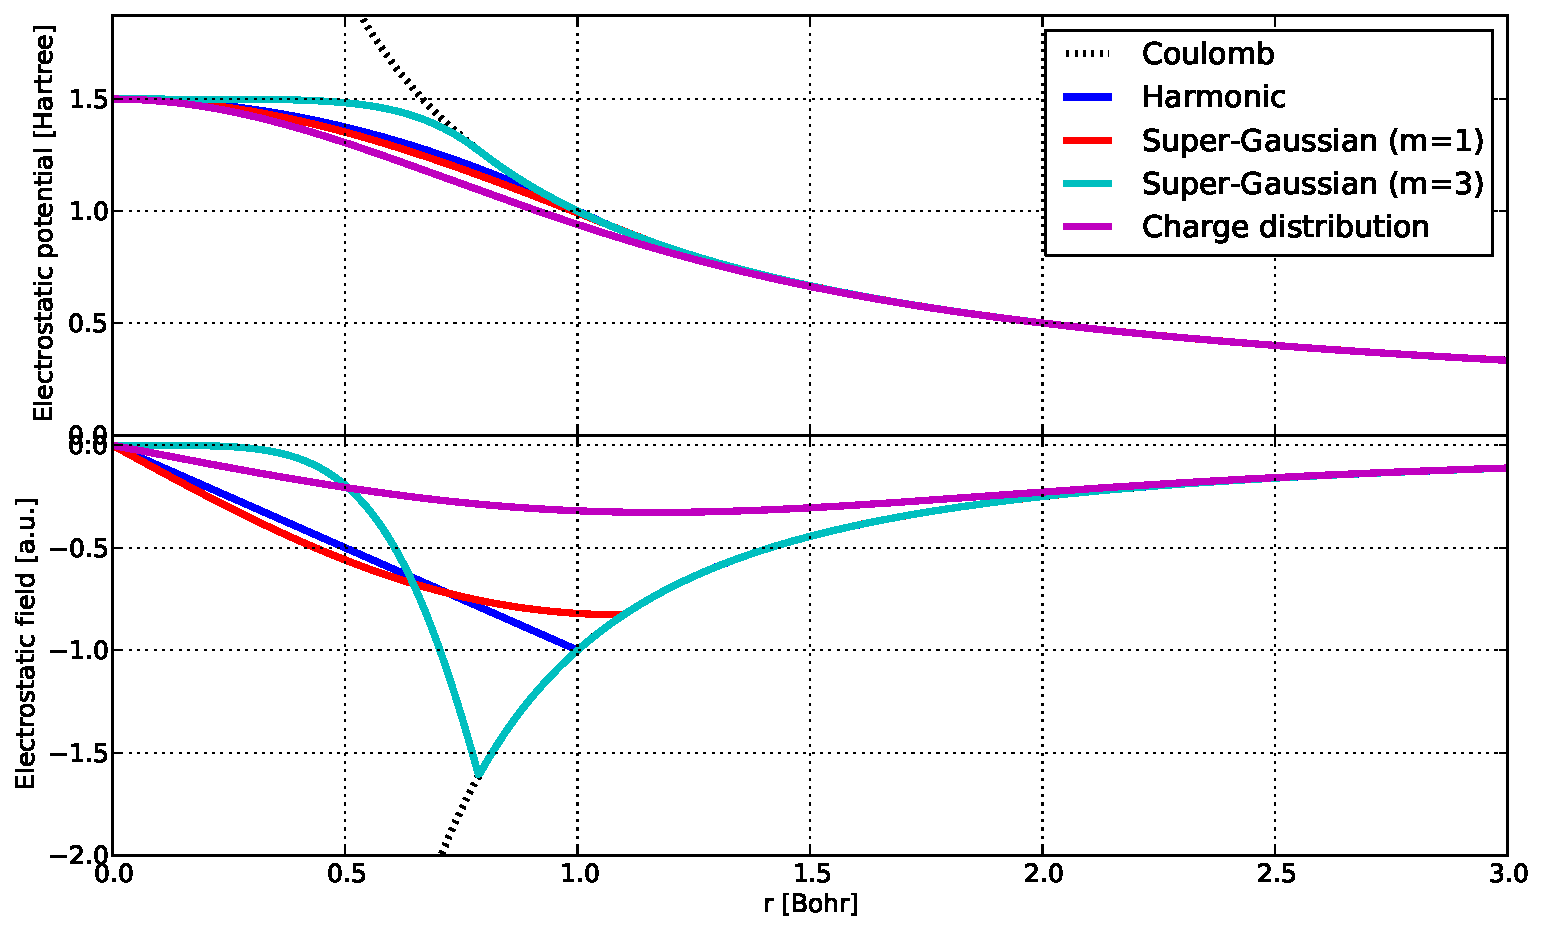
\includegraphics[width=0.98\columnwidth]{figures/potential_shapes}
    \end{center}
    \caption{\label{fig:potential:shapes}Potential shapes and their respective
electric field. Note the use of atomic units and $\phi_0$ = 1.5 Hartree.}
\end{figure}

It was found that the potential given by the charge distribution of equation
\eqref{eqn:md:smoothed:phi} and the associated electrostatic field of
\eqref{eqn:md:smoothed:E} give the less numerical heating. As explained
previously, the time discretization used to integrate the equations of motion
assume that the change in force between two time steps is linear. As can be
seen on figure \ref{fig:potential:shapes}, the charge distribution curve
(magenta) does not have a discontinuity and is therefore the prefered one.

To validate the selection of the smoothing curve, photo-ionization was forced
on a single atom and the total energy tacked. In this ionization case, the
electron comes out of the ion with a maximum of kinetic energy. It is thus a
good candidate to test if numerical heating is present or not. If the total
energy is conserved, then the selected parameters (potential depth, smoothing
curve and time step) can be used with good confidence. Figure
\ref{fig:potential:heating} shows numerical heating.

\emptyfig{NUMERICAL HEATING}{fig:potential:heating}


\subsubsection{Implementation details}

Our group previously used Barnes and Hut treecode implementation,
freely available\cite{treecode} through the GPL version 2. The code was adapted
to simulate charged particles (Coulomb force) instead of masses (gravitational
force) with some ionization routines added (see for example reference
\cite{Jungreuthmayer2005}). While reducing development time by re-using already
written code, the maintenance burden introduced by many factors (initial
implementation written in the C language, usage of global variables
throughout the code, multiple coding styles from different people throughout
the years, lack of vision, lack of revision control system to give the freedom
of deleting code from the active version without loosing the ability to roll
back, many subtle and important bugs, stability issues, etc.) pushed the author
to restart from scratch. This allowed using modern development techniques to be
used. For example, all development was done through a revision control system
(subversion\cite{svn} at first, then switched to git\cite{git}) in the C++
language instead of C. The object oriented nature of C++ allowed encapsulation
of different parts of the code which could then be tested and validated
individually. This gave better flexibility to the code, a required asset to
push further the development of features.

A substantial number of MD packages are freely available and were
their usage was considered instead of re-implementing a new one from scratch.
Examples are GROMACS\footnote{GROMACS:
\url{http://www.gromacs.org/}} or NAMD\footnote{NAMD:
\url{http://www.ks.uiuc.edu/Research/namd/}}. A major issue with these
pre-existing MD packages is their target audience; they aim to simulate large
bio-molecules with mostly short range interactions. Another important problem
is the number of particles throughout the simulations; while many packages
assume a constant number of particles, the present work required creating
(ionization) and annihilating (recombination) particles throughout simulations.
Controlling the MD part of the code allowed better integration of the
ionization aspects.

Other MD packages were not mature enough or simply non-existent at the time.
For example the largely used HOOMD-blue\footnote{HOOMD-blue:
\url{http://codeblue.umich.edu/hoomd-blue/}} which uses extensively
Nvidia GPUs released its first version (v0.6.0) in February 2008.
Additionally, the knowledge and experience gained by writing from scratch such
a package is invaluable.






\subsubsection{Quantum FDTD (QFDTD)}
One model proposed to explain the high charge states seen in some experiments
is the lowering of the ionization barrier, used in conjunction with classical
MD simulations. This model assumes that an electron can be inner ionized when
the potential of a neighbouring ion lowers the potential of the electron's
parent ion. If this barrier is lowered enough so that it drops below the
electron's energy level, the electron becomes free to leave the ion and evolve
in the cluster environment. An open question is how close this model, used
with a classical MD, is to reality. Special care needs to be taken when a
particle, evolving in a quantum world, is to be treated classically. How does
the bound electron's wavefunction reacts to the presence of a second ion
perturbing the potential? Is the wavefunction really evolving into a state
where we can say the electron is shared by the two ions? If the electron is
really shared by the two ions, can we classically let it evolve inside the
cluster environment?

These questioned pushed us to look at the quantum aspects in more details. Many
different tools exist to calculate the ground state of system, even with
multiple electrons, as describe previously. Additionally, excited states are
capital in ACI and as such we wanted a tool that could give us information not
only on the ground state but also on excited states.

After stumbling on an interesting article that used the Finite-Difference
Time-Domain (FDTD) algorithm to solve \schrodinger equation\cite{Sudiarta2007}
it was decided to explore this idea since not much work could be found on this
\textit{Quantum FDTD} (QFDTD) method and due to previous experiences
implementing electrodynamics FDTD.

FDTD is an (old) algorithm developed in 1966 by Yee\cite{Yee1966} to solve
Maxwell's equation on a grid using a leap-frog integration. The number of
scientific articles using FDTD has exponentially increased since the '80s
largely due to the increase in computation resources. Indeed, a three
dimensional grid with the three vector components of both the electric and
magnetic fields requires huge amount of memory that were definitely not present
in the late '60s. The reader is invited to read the excellent book on FDTD by
Allen Taflove and Susan Hagness\cite{Taflove2005} covering 40 years of FDTD
development in electrodynamics simulations.

Other simulation techniques like Finite-Element Methods (FEM) or Finite-Volume
Methods (FVM) can be seen as more complex then Finite-Differences Methods
(FDM). This gives some elegance and simplicity in the FDM algorithms.
Additionally, since FDTD is an explicit algorithm, implementations are
generally easy and efficient and the local nature of the algorithm makes it
easily parallelizable on distributed memory systems.

Sullivan was the first to apply the FDTD method to solve the \schrodinger
equation in his 2000 book\cite{Sullivan2000} where he obtains the wavefunction
of an electron hitting a potential barrier. Latter in 2001 he used the FDTD
method to simulate one and two electrons in a quantum dot\cite{Sullivan2001}.
The Hartree-Fock approximation was used to describe the two electrons problem
and thus required the use of Fourier transforms to calculate the Coulomb
and exchange terms. Due to this extra required calculation, the problem was
restricted to two dimensions only. The following year, he introduced a method
to calculate the eigenstates of an arbitrary system using
FDTD\cite{Sullivan2002}. This method requires two distinct simulations: the
first one finds the eigenvalues and the second one stores the states
corresponding to these eigenvalues, doubling the simulation time required.
The interaction with a magnetic field was included through the vector potential
and later\cite{Sullivan2003,Sullivan2004} used to calculate spin interaction.
Only in 2005 did the first three dimensional
simulations\cite{Sullivan2005a} were performed as proof of concept; only a
single electron was simulated. Eigenstates and eigenvalues were obtained for an
example quantum well as well as a two ions system. A more complicated three
dimensional system was later simulated in \cite{Sullivan2005b}, still with a
single electron.

Later Sudiarta suggested\cite{Sudiarta2007} a new way to use the FDTD method to
solve the \schrodinger equation for a single electron system. By switching to
\textit{imaginary time}, \schrodinger equation can be solved more easily and
more efficiently to get the eigenvalues and eigenstates of the system. It was
later shown that the interaction with a magnetic field could also be added to
the imaginary-time method\cite{Sudiarta2008} and that FDTD could be used to
construct the thermal density matrix of single particle\cite{Sudiarta2009}.

Due to the explicit nature of the FDTD algorithm (values can be obtained at the
next time step from values at the current time step only) the method is
conditionally stable; an upper bound on the time step size must be taken. The
Courant-Friedrichs-Lewy (CFL) condition gives the upper bound. Dai \textit{et
al.} derive\cite{Dai2005} the stability condition for a constant in time
potential:
\begin{align}
\Delta t < \frac{2}{
    \frac{2 \hbar}{m} \pa{
         \frac{1}{\Delta x}
        +\frac{1}{\Delta y}
        +\frac{1}{\Delta z}
        }
        + \textrm{max}\abs{V\pa{\vr}} / \hbar
    }
\end{align}


Both real-time and imaginary-time methods were implemented. Let's describe the
two algorithms.

First, let's define the time dependent \schrodinger equation describing a
wavefunction $\psi$ inside a potential $V$:
\begin{align}
\im \hbar \delt{  } \ket{\psi\pa{\vr, t}}
    & = \pa{-\frac{\hbar^2}{2 m} \laplacian{} + V\pa{\vr, t} } \ket{\psi\pa{\vr,
t}}
\label{eqn:schrodinger:si}
\end{align}
To ease the calculation, let's switch to atomic units where $\hbar = 1$ and $m
= 1$:
\begin{align}
\im \delt{  } \ket{\psi\pa{\vr, t}}
    & = \pa{-\frac{1}{2} \laplacian{} + V\pa{\vr, t} } \ket{\psi\pa{\vr, t}}
\label{eqn:schrodinger:au}
\end{align}
At initial time $t = 0$, the wavefunction $\ket{\psi\pa{\vr, t}}$ is
decomposed into its eigenstates basis:
\begin{align}
\ket{\psi\pa{\vr, t=0}} & = \sum_{n=0}^{\infty} c_n \ket{\phi_n\pa{\vr}}
\label{eqn:wavefunction:real:initial}
\end{align}
The time-evolution operator (or propagator) $\oU\pa{t}$ is, in atomic units:
\begin{align}
\oU\pa{t} & = \ex{ - \im t \oH }
\label{eqn:propagator:real}
\end{align}
and when applied to the initial state \eqref{eqn:wavefunction:real:initial}
gives the time evolution of the wavefunction:
\begin{align}
\oU\pa{t} \ket{\psi\pa{\vr, t=0}}
    = \ket{\psi\pa{\vr, t}}
  & = \e{ - \im t \oH } \sum_{n=0}^{\infty} c_n \ket{\phi_n\pa{\vr}}
\end{align}
Since the operator $\oH$ applied to the eigenstates
$\ket{\phi_n\pa{\vr}}$ gives the eigenvalues $E_n$, the previous equation
becomes:
\begin{align}
\ket{\psi\pa{\vr, t}}
 & = \sum_{n=0}^{\infty} \e{ - \im t E_n } c_n \ket{\phi_n\pa{\vr}}
\label{eqn:wavefunction:eigenstates:time_evolution:real}
\end{align}
The time evolution of each eigenstates is thus an oscillation between their real
and imaginary parts of which the frequency is given by the eigenvalue $E_n$.



Equation \eqref{eqn:schrodinger:au} can now be solved either in real-time or
imaginary-time, the former being explained first.

Let's separate the real and imaginary components of equation
\eqref{eqn:schrodinger:au} (simplifying the notation):
\begin{align}
\im \delt{  } \pa{ \psi_R + \im \psi_I}
    & = \pa{-\frac{1}{2} \laplacian{} + V }
        \pa{ \psi_R + \im \psi_I} \\
\im \delt{  } \psi_R - \delt{  } \psi_I
    & = \pa{-\frac{1}{2} \laplacian{} + V } \psi_R
      + \im \pa{-\frac{1}{2} \laplacian{} + V } \psi_I
\end{align}
giving two equations describing the time evolution of two effective fields:
\begin{subequations}
\begin{align}
\delt{  } \psi_R & =   \pa{-\frac{1}{2} \laplacian{} + V } \psi_I
\label{eqn:schrodinger:real:real} \\
\delt{  } \psi_I & = - \pa{-\frac{1}{2} \laplacian{} + V } \psi_R
\label{eqn:schrodinger:real:imag}
\end{align}
\label{eqn:schrodinger:real}
\end{subequations}
The real and imaginary parts in equation \eqref{eqn:schrodinger:real} can be
compared to the electric and magnetic fields in the traditional electrodynamics
FDTD method. The integration is performed using a leap-frog scheme. We
first define $\psi_{i,j,k}^{n}$ the wavefunction located at the grid cell
$\pa{i,j,k}$ and at time step $n$. Then equation equation
\eqref{eqn:schrodinger:real:imag} is evaluated at time step $n$ and, using
(second order) central-differences, we get:
\begin{align}
\left. \delt{  } \psi_I \right|_{n}
& = \left. - \pa{-\frac{1}{2} \laplacian{} + V^{n} } \psi_R \right|_{n} \\
\frac{\psi_{I}^{n+1/2} - \psi_{I}^{n-1/2}}{\Delta t}
& = - \pa{-\frac{1}{2} \laplacian{} + V^{n} } \psi_{R}^{n} \\
\psi_{I}^{n+1/2}
& = \psi_{I}^{n-1/2} - \Delta t \pa{-\frac{1}{2} \laplacian{} + V^{n} }
\psi_{R}^{n}
\label{eqn:schrodinger:real:imag:discretized}
\end{align}
Similarly, defining the time derivative in \eqref{eqn:schrodinger:real:real} at
time step $n$ and again using (second order) central-differences:
\begin{align}
\left. \delt{  } \psi_R \right|_{n+1/2}
& = \left. \pa{-\frac{1}{2} \laplacian{} + V^{n} } \psi_I \right|_{n+1/2} \\
\frac{\psi_{R}^{n+1} - \psi_{R}^{n}}{\Delta t}
& = \pa{-\frac{1}{2} \laplacian{} + V^{n} } \psi_{I}^{n+1/2} \\
\psi_{R}^{n+1}
& = \psi_{R}^{n} + \Delta t \pa{-\frac{1}{2} \laplacian{} + V^{n} }
\psi_{I}^{n+1/2}
\label{eqn:schrodinger:real:real:discretized}
\end{align}

Lastly, the Laplacian is discretized on a grid using (second order)
central-differences:
\begin{align}
\laplacian{} \psi_{i,j,k}^{n} \approx
      \frac{ \psi_{i+1,j,k}^{n} - \psi_{i-1,j,k}^{n} }{2 \Delta x}
    + \frac{ \psi_{i,j+1,k}^{n} - \psi_{i,j-1,k}^{n} }{2 \Delta y}
    + \frac{ \psi_{i,j,k+1}^{n} - \psi_{i,j,k-1}^{n} }{2 \Delta z}
\label{eqn:laplacian:discretized}
\end{align}

Equations \eqref{eqn:schrodinger:real:imag:discretized},
\eqref{eqn:schrodinger:real:real:discretized} and
\eqref{eqn:laplacian:discretized} are then used to propagate in time the real
and imaginary components of the electronic wavefunction. Note that, contrary
to the Yee cell in the electrodynamics FDTD, the two components of the
wavefunction don't have to be defined at different location inside the grid
cell; they are defined at the same location as shown on figure
\ref{fig:qfdtd:cell}.

\emptyfig{YEE CELL VS QFDTD CELL}{fig:qfdtd:cell}

Equations \eqref{eqn:schrodinger:real:imag:discretized} and
\eqref{eqn:schrodinger:real:real:discretized} by themselves only describe the
time evolution of a wavefunction inside a potential; it does not give a direct
way to obtain the eigenstates of an Hamiltonian. Different approaches exist to
obtain these; Sullivan describes some of them. Eigenvalues though are
relatively easy to obtain though.

By numerically propagating in time a wavefunction $\psi$ using equations
\eqref{eqn:schrodinger:real:imag:discretized} and
\eqref{eqn:schrodinger:real:real:discretized} the system's eigenstates will
evolve according to equation
\eqref{eqn:wavefunction:eigenstates:time_evolution:real}. This evolution is an
oscillation between real and imaginary part at a specific frequency; the states'
eigenvalue. By taking a Fourier transform of the time evolution, eigenvalues
can be identified on a power spectrum. The published article of section
\ref{section:papers:qfdtd} describes a novel method of extracting the
eigenvalues of all eigenstates present in the simulated wavefunction $\psi$.



The second QFDTD method, called the \textit{imaginary-time} method, differs in
that it first requires that the potential be constant in time ($V\pa{\vr, t}
\rightarrow V\pa{\vr}$). Further, a Wick rotation is performed in time ($\im t
\rightarrow \tau$) and the \schrodinger equation in imaginary time is
obtained:
\begin{align}
- \deli{}{\tau} \ket{\psi\pa{\vr, \tau}}
    & = \pa{-\frac{1}{2} \laplacian{} + V\pa{\vr} } \ket{\psi\pa{\vr, \tau}}
\label{eqn:schrodinger:imaginary}
\end{align}
Note that equation \eqref{eqn:schrodinger:imaginary} is not complex and is
similar to the heat equation.


Contrary to the real-time method, the ``time'' evolution of the imaginary
method is not oscillatory. Indeed, the propagator of equation
\eqref{eqn:propagator:real} becomes, in imaginary time:
\begin{align}
\oU\pa{\tau} & = \ex{ - \tau \oH } \label{eqn:propagator:imag}
\end{align}
and the wavefunctions evolution becomes:
\begin{align}
\ket{\psi\pa{\vr, \tau}}
 & = \sum_{n=0}^{\infty} c_n \e{ - \tau E_n } \ket{\phi_n\pa{\vr}}
\end{align}
The imaginary time evolution is thus an exponential growth with the different
eigenstates having different growth rates. It thus becomes possible to isolate
the different eigenstates from each other. A novel method to isolate these
states is described in the published article of section
\ref{section:papers:qfdtd} (page \pageref{section:papers:qfdtd}).

Because equation \eqref{eqn:schrodinger:imaginary} is real, a single scalar
field needs to be discretized on the grid. The discretization is similar to the
real-time method: equation \eqref{eqn:schrodinger:imaginary} is evaluated at
time step $n$ and the time derivative is discretized, in this case using (first
order) forward-differences (and again simplifying the notation):
\begin{align}
- \left. \deli{}{\tau} \psi \right|_{n}
    & = \cro{ \pa{-\frac{1}{2} \laplacian{} + V} \psi }_{n}
\\
\frac{\psi^{n+1} - \psi^{n}}{\Delta \tau}
    & = \pa{\frac{1}{2} \laplacian{} - V} \psi_{n}
\\
\psi^{n+1} & = \cro{1 + \Delta \tau \pa{\frac{1}{2} \laplacian{} - V}} \psi^{n}
\label{eqn:schrodinger:imaginary:discretized}
\end{align}
The Laplacian is discretized with equation \eqref{eqn:laplacian:discretized}.
Since a single scalar field is used to describe $\psi$, special care needs to
be taken in the code implementation. Indeed, equation
\eqref{eqn:schrodinger:imaginary:discretized} uses the Laplacian of the
wavefunction at the previous time step $n$ to update the wavefunction to
time step $n+1$. For example, calculating $\psi^{n+1}_{i,j,k}$ requires
$\psi^{n}_{i-1,j,k}$ and $\psi^{n}_{i+1,j,k}$ (for the $x$ derivative in the
Laplacian) but when calculating the next value in $x$ ($\psi^{n+1}_{i+1,j,k}$)
the required values are now $\psi^{n}_{i,j,k}$ and $\psi^{n}_{i+2,j,k}$, the
former being already updated. The easiest and simplest way to solve this
dependency problem is to store two grids; one for $\psi^{n}$ and another for
$\psi^{n+1}$, alternating between them when calculating equations
\eqref{eqn:schrodinger:real:imag:discretized} and
\eqref{eqn:schrodinger:real:real:discretized}.





\subsubsection{Acceleration through OpenCL and GP-GPUs}
A new trend lately in High Performance Computing (HPC) is code acceleration
through graphics cards. Similar to the ubiquitous Moore's Law in the CPU world,
video cards power evolved exponentially during the last twenty years, pushed
by the never ending need of more realistic video games. From ``dumb'' devices
drawing primitive shapes on a display, they evolved to extremely powerful
devices and started to act more like CPU by being programmable (shaders) during
the first half of 2000. The term \textit{Graphical Processing Unit} (GPU) was
coined in 1999 by Nvidia, the biggest vendor of video cards, as a selling point
to their product and to emphasize the fact that their chips were becoming more
and more alike CPUs.

Due to this increase in power, people tried to use these video cards as
accelerators for other things than real video operations. Because GPUs have
intrinsically high parallelism (for example the same operation is performed on
all pixels of an image in parallel) HPC users and developers got interested.
In his 2005 book, Taflove described a way to use a video card's GPU to
accelerate his electrodynamics FDTD solver \cite{Taflove2005}. At that time no
General-Programming GPU (GP-GPU) framework existed so Taflove (and anyone
interested in using GPUs at that time) had to ``translate'' the FDTD algorithm
into one that could be understood by a video card. This process was extremely
hard as it required using low level graphic primitives; in his case, OpenGL
calls. Normally OpenGL is used to draw animated scenes on the user's screen.
Notable examples of OpenGL usage is video games where the user is immersed in a
virtual three dimensional space. The process of re-writing an algorithm into
OpenGL calls is one that only a few highly skilled and knowledgeable people can
tackle.

In 2007, Nvidia saw an opportunity for market expansion. Why not let
non-videogames programmer use the powerful GPUs for something else then video
operations? For this to happen, a programming framework had to be released; the
amount of programmers and scientists able to exploit OpenGL to their advantage
was limited. They thus released their \textit{Compute Unified Device
Architecture} (CUDA), later just renamed CUDA. CUDA allows writing normal C or
C++ programs with some extensions, called \textit{kernels}, that can be run on
the GPU. These kernels have the same structure as C functions but are executed
concurrently by every cores on the GPU\footnote{Technically, GPUs don't have
``cores'' \textit{per se} like CPUs but the comparison can still be made.}. The
number of cores on a recent consumer grade video card is now of the order of
many hundreds; a 50\$ Nvidia GT 620 has 96 CUDA cores and 1 GB of RAM, while the
GTX TITAN has 2688 CUDA cores and 6 GB but cost more than 1,000 \$. Even though
the highest priced GPU can be more expensive than complete workstations, no CPUs
can offer close to three thousand cores for a still affordable price.

A year after CUDA was released, Apple wanted a framework that would allow
programs to be accelerated on their top-of-the-line product's GPU while still
being able to run on their lower-end range of products (which did not have a
discrete video card). Additionally, some Apple products were released with ATI
video cards (Nvidia's main competitor) which, understandably, never supported
CUDA. They thus released a framework called \textit{OpenCL} (standing for
Open Compute Language) in 2008 with the help of many partners (IBM, ATI, Intel
and even Nvidia). While conceptually similar to CUDA (smaller routines are
written in a kernel function and launched individually on the GPUs by the main
program) OpenCL has the advantage of targeting heterogeneous platforms
consisting of (possibly and not limited to) many CPUs, many cores and GPUs. The
main advantage of OpenCL is its portability; a program written in OpenCL can
not only run on GPUs from ATI and Nvidia but also on traditional CPUs,
exploiting all cores available on the CPUs transparently.

It was thus decided to port the two codes (MD and QFDTD) to OpenCL to take
advantage of the GPU power while retaining portability.

Some things are important to consider when porting codes to GPU frameworks.
First, because a core on a GPU is quite slower than a core on a CPU,
parallelisms must be extracted from algorithms. Second, the main drawback of
GP-GPU programming is the fact that GPUs have their own memory, independent of
the system's memory; kernels will only have access to the device's memory. Data
required for kernel calculation must thus be first transferred to the device's
memory and similarly the resulting data must be transferred back to the host
memory where it can be further processed by the rest of the main program. Video
cards today are connected to a computer through PCI-Express (PCIe) connections.
While fast, it can still be a bottleneck if data is to be transferred back and
forth similarly to main memory. It is thus necessary to reduce to a minimum the
data transfer between the host and the device, similarly to communications in a
distributed memory parallel programming paradigm.

In the case of the MD algorithm, every interaction pair is independent of all
others and can thus be calculated concurrently; this is thus the basis of the
OpenCL implementation. The main loop that calculates the electrostatic field
and potential at every particle's position is implemented as an OpenCL kernel.
Each thread on the GPU will thus calculate the interaction between one particle
and all others. Once the MD kernels are launched on the GPU, they are only
halted when either ionization is to be calculated (at each femtoseconds) or
when data needs to be saved (to take a snapshot of the simulation for example).
This prevent the GPU from being interrupted too often and reduces the amount of
data transfers. Using this OpenCL implementation, MD simulations could be run
80 times faster than on conventional CPUs.

As for the QFDTD, only the real time algorithm was implemented as OpenCL
kernels since the imaginary time method did not require long simulation times.
As in the case of the MD, the real time algorithm is left running on the GPU
until data needs to be saved to a snapshot or post-processed to reduce
transfers.




\subsubsection{Libraries}

Additionally, a total of seven other libraries were developed to support some
generic features of the code. These libraries are:
\begin{itemize}
\item ionization.git\footnote{ \url{
    https://gitlab.cphoton.science.uottawa.ca/nbigaouette/ionization}}:
    All ionization routines described in section
    \ref{section:intro:clusters:heating}
\item timing.git\footnote{ \url{
    https://gitlab.cphoton.science.uottawa.ca/nbigaouette/timing}}:
    Timing routines used to measure running time, estimated time of arrival
(ETA), etc.
\item stdcout.git\footnote{ \url{
    https://gitlab.cphoton.science.uottawa.ca/nbigaouette/stdcout}}:
    Logging features allowing saving the output of any simulations to a log
    (compressed) file.
\item prng.git\footnote{ \url{
    https://gitlab.cphoton.science.uottawa.ca/nbigaouette/prng}}:
    Pseudo-random number generator (PRNG) library. Wrapper around
dSFMT\cite{prng2009}. Defines easy to use PRNG functions, distributions, seed,
etc. Keeps track of how many times it has been called for easy reloading
exactly where simulation left off.
\item memory.git\footnote{ \url{
    https://gitlab.cphoton.science.uottawa.ca/nbigaouette/memory}}:
    Wrappers around malloc() and calloc() that will automatically check that
    the allocation succeeded. Will also keep track of the amount of
    memory allocated and allow setting a maximum value, preventing
    over-allocation due to bugs or user errors. Can also print values directly
    in binary for easy debugging.
\item io.git\footnote{ \url{
    https://gitlab.cphoton.science.uottawa.ca/nbigaouette/io}}:
    Input and Output library. Wrappers around TinyXML library\cite{tinyxml} for
reading input file. Wrappers around NetCDF\cite{netcdf} for self-contained
output files, used in simulation snapshots.
\item libpotentials.git\footnote{ \url{
    https://gitlab.cphoton.science.uottawa.ca/nbigaouette/libpotentials}}:
    Functions implementing and abstracting different potential shapes.
\item oclutils.git\footnote{ \url{
    https://gitlab.cphoton.science.uottawa.ca/nbigaouette/oclutils}}:
    Library to ease the use of OpenCL devices. Allows selecting the best GPUs
    available on a workstation and locking it to prevent other simulations from
    using it.
\item get\_libraries.git\footnote{ \url{
    https://gitlab.cphoton.science.uottawa.ca/nbigaouette/get_libraries}}:
    Simple script that will download all the previous required libraries,
    compile them and install them in the user's directory.
\end{itemize}
A detailed guide on the compilation and usage of the simulation package can be
read in appendix \ref{appendix:code}.


\subsection{Thesis Outline}
Don't forget a review/description of each sections of the thesis.



\ReferencesSubsection{references_intro}
